\section{Introduction}
\label{sec:intro}

\begin{comment}
-- OUTLINE
a. Define counterfactual. counterfactuals are how we understand stuff (cite psychology papers) and run decent experiments. Counterfactuals are hard in the real world (cite pearl), but easy if we're analyzing a model
b. Current counterfactuals in NLP: useful for training and eval (contrast sets), but done by hand. Too much work, relies on creativity, may miss stuff. For explanations: adversarial examples, or simple word substitutions.
c. We formalize the task of counterfactual generation: given x, produce \xp, and then rank according to the task. We train a model to do this (some detail).
d. we apply the model to training, eval, explanations. summary of results. Important: compare to counterfactuals created by hand, this is better and faster
\end{comment}

\begin{figure}[t]
\centering
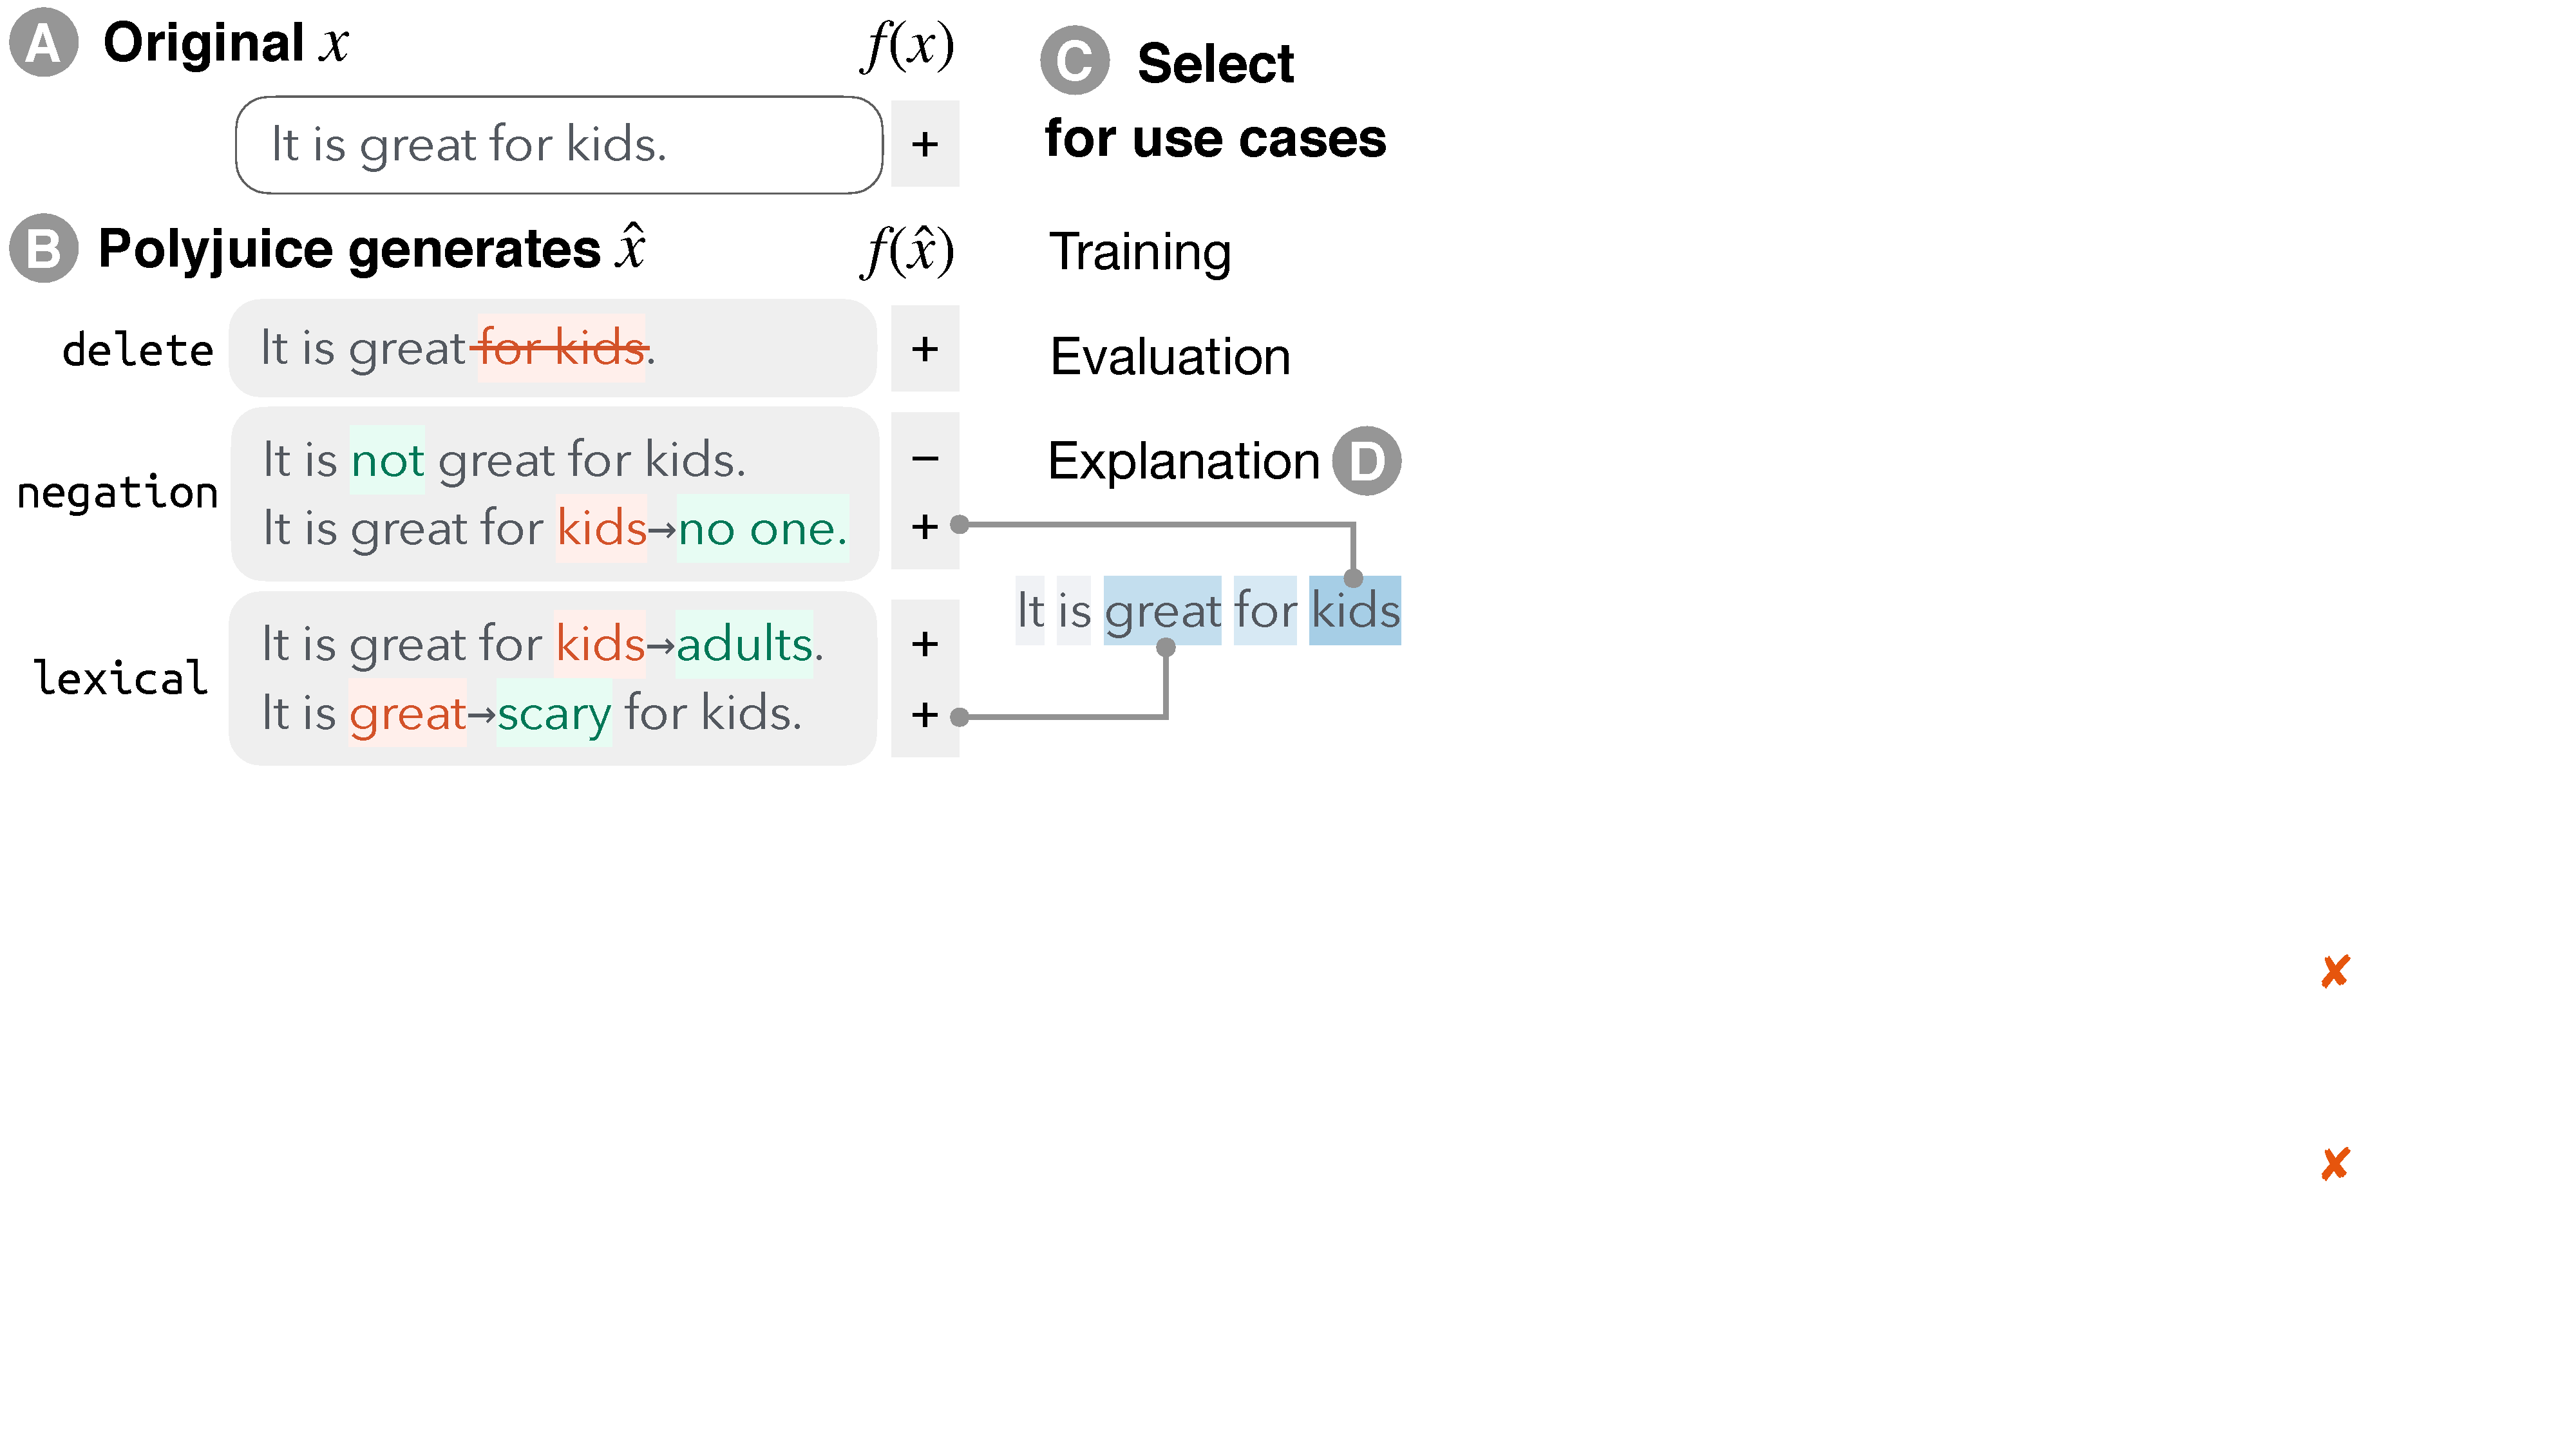
\includegraphics[trim={0 18cm 30.5cm 0cm},clip, width=1\columnwidth]{figures/teaser.pdf}
\vspace{-15pt}
\caption{
Overview: given an original sentiment analysis instance $x$ (A), \sysname generates (B) a large number of $\xp$, which are then (C) independently selected for downstream use cases.
For example, in (D), we select $\xp$ as counterfactual explanations, based on whether they complement the feature attributions: though both ``great'' and ``kids'' are deemed important, the selected $\xp$ show that perturbing them may not affect the prediction $f(x)=f(\xp)=\text{\emph{positive}}$, revealing model errors.
}
\vspace{-15pt}
\label{fig:teaser}
\end{figure} 
 

Counterfactual reasoning --- mentally simulating what \emph{would have happened} if conditions were different --- is a common tool for making causality assessments~\cite{kahneman}, which in turn are crucial for model training, evaluation, and explanation~\cite{miller}. 
For example, in Figure~\ref{fig:teaser}, \exinline{It is great for kids} is perturbed into multiple variations, and each variation brings a unique insight by simulating what would have happened if the sentence was different.

%\hao{suggestion: it could be great if you can highlight the high cost of existing approaches by being more specific on, e.g., the cost of human annotation and cite some works backing it up. something like the human annotation in xxx costs xxx money/time would be very convincing. }
Applications of counterfactual reasoning to Natural Language Processing (NLP) generally specify the relationship $x \veryshortarrow \xp$, and then create $\xp$ according to the relationship.
As a result, generation methods are heavily constrained by the application, each having their own limitations.
For example, a minimal edit of a sentence $x$ that results in a different label is useful for model training and evaluation.
Such $\xp$ are usually gathered with human efforts, \ie human annotators manually create counterfactuals~\cite{gardner2020contrast} or perturbation functions that generate counterfactuals~\cite{wu2019errudite}.
These are costly to generate --- taking 4-5 minutes per counterfactual~\cite{kaushik2019learning} --- and may miss important patterns due to their reliance on human intuition (\eg humans may cover \swap{great}{not great}, but can easily miss \swap{kids}{no one} in Figure~\ref{fig:teaser}B).
%Though it is cheaper to automate the process with parsing templates~\cite{li2020linguistically}, the templates usually have limited coverage on either the patterns-to-perturb, or the applicable data points.
Adversarial examples are a different form of counterfactual reasoning: $x$ and $\xp$ have different model predictions \emph{despite} being minimally edited and semantically equivalent --- the latter limiting most perturbations to be automated word replacements or other forms of paraphrasing~\cite{iyyer2018adversarial, ribeiro2018semantically}.

However, we observe that generation methods do not have to be isolated, as various applications share similar requirements on $x\veryshortarrow\xp$ (\eg minimal edits).
In fact, the exhaustive search of automated methods can cover the training and evaluation more comprehensively, and non-paraphrasing changes like \emph{add negation} are valuable adversarials for tasks like named entity recognition. 
%\hao{might be good to clarify that these two are not mutually-exclusive: adversarial examples should sometimes be close to the original}

In this work, we formalize the task of \emph{automatic counterfactual generation}, which disentangles the generation from the application (\S\ref{sec:general_purpose}).
First, in generation, given an input $x$, we produce a set of counterfactuals $\hat{\xset} = \{\xp_1, \xp_2, ...\}$ with reasonable but \emph{application-agnostic} relationships $x \veryshortarrow \xp_i$ (Figure~\ref{fig:teaser}B).
We require the counterfactuals to be \emph{fluent}, \emph{diverse}, and \emph{close to $x$}.
Afterwards, we use \emph{application-specific} selection methods to find subsets of $\xp$ that are most effective for the applications of interest (Figure~\ref{fig:teaser}C).
We frame the generation step as text generation, and finetune GPT-2~\cite{radford2019language} into a generator called \emph{\sysname} using datasets of $(x, \xp)$ pairs. 
We also allow for targeted counterfactuals, by specifying where the perturbation occurs in the sentence~\cite{donahue2020enabling} and using \tagstrs such as \ctrltag{negation} or \ctrltag{delete} (Figure~\ref{fig:teaser}B).
By scaling up the generation beyond human intuitions and simple paraphrasing, \sysname helps more effectively allocate human efforts to the \emph{verification, labeling, and analyses on the counterfactual instances.}

%\hao{suggestions: merge the following paragraphs (which are tedious to read), trim the less interesting details, and highlight the results that are exciting.}
We propose simple yet effective selection strategies, and show that a single \sysname model can team up with humans to support multiple downstream applications:
(1) it can \emph{facilitate counterfactual training and evaluation} (\S\ref{sec:app_label}). 
\wts{Add the range of the number here.}
By asking humans to \emph{label} a set of \emph{unique} counterfactuals, we produce high-quality contrast sets~\cite{gardner2020contrast} at a fraction of the annotation effort compared to creating them from scratch~\cite{kaushik2019learning}.
We similarly produce training data that improves model generalization in three classification tasks. %, when compared to adding the same amount of non-counterfactual data.
(2) \sysname supports \emph{producing black-box counterfactual explanations} (\S\ref{sec:app_explain}), as in Figure~\ref{fig:teaser}D.
%Such explanations have been elusive in NLP, despite evidence from social science research~\cite{miller} indicating that they may be more intuitive, or may complement feature attribution or attention maps.
% We prioritize counterfactuals with \emph{abnormal} model behaviors, \ie the actual changes in prediction do not match the expectation.
%(measured by sentence similarity or perturbed feature weights.)
%We select \sysname counterfactuals \emph{that potentially highlight mistaken model predictions}, as in Figure~\ref{fig:teaser}D.
%An example would be Figure~\ref{fig:teaser}D: the model incorrectly predicts \emph{positive} after \swap{kids}{no one} in Figure~\ref{fig:teaser}D, even though ``kids'' is supposed to be important.
In a user study, expert users only did slightly better than random (accuracy: $55 \pm 6\%$) at predicting what a model would do on \sysname counterfactuals that are selected to \emph{highlight mistaken model predictions}, even after inspecting the models based on state-of-the-art explanation methods.
% In fact, the explanations found more bugs within spots where users considered inspected after
(3) \sysname also helps \emph{support more systematic error analysis} by highlighting inspection spots easily missed by human analysts. 
These indicate that such counterfactuals can complement existing explanation and analysis methods, echoing evidence from social science~\cite{miller}. 

In summary, we:

\begin{compactenum}
\item  Formalize the general-purpose counterfactual generation task. 
By \emph{separating the generation from the use cases}, we generate fluent and diverse counterfactuals that bypass application-specific constraints.
%. \hao{maybe emphasize the benefits of this}
\item Finetune a generator called \sysname, by collecting paired sentences and enhancing controls with infilling structures and \tagstrs --- the control is \emph{the backbone of} various downstream applications.
%\sysname generates plausible and diverse counterfactuals, with control over where perturbations happen and what they do.
The model is at \modelurl.
%, and we plan to opensource the selection strategies.
\item Apply \sysname to \emph{model training, evaluation, and explanation}, using various selection methods (which we will opensource).
\sysname helps collect high-quality training and evaluation data with 40\% less annotation effort, and find model bugs that on top of feature attribution explanations and counterfactual analysis.
\end{compactenum}
\wts{Maybe can delete if we run out of space.}


% we observe that \sysname explanations can complement popular feature attribution methods and highlight their blind spots.
% After viewing SHAP weights~\cite{NIPS2017_7062} and interacting with the model, experts still could not predict model behaviors on counterfactuals selected for explanations, and missed 5\% and 25\% more cases than the human-generated or random baselines.
